%%%%%%%%%%%%%%%%%%%%%%%%%%%%%%%%%%%%%%
% Contribution to IKP annual report 2021
%%%%%%%%%%%%%%%%%%%%%%%%%%%%%%%%%%%%%%
\documentclass[fleqn,twocolumn,a4paper]{ikpar}
\usepackage{hyperref}
\usepackage{paralist}
\usepackage{times,mathptm}
\usepackage{graphicx}
\usepackage{caption}
\usepackage{subfig}
\usepackage{gensymb}
\pagestyle{empty}

% standadized SI units
\usepackage[per-mode=symbol, range-units=single, binary-units=true]{siunitx}
\DeclareSIUnit\clight{\text{\ensuremath{c}}} % redefine light speed symbol
\DeclareSIUnit\momentum{\GeV\per\clight} % momentum in GeV/c
\DeclareSIUnit\tmom{(\momentum)^2} % 4-momentum squared
\DeclareSIUnit\atom{\text{atoms}} 
\DeclareSIUnit\event{\text{events}} 

% \addtolength{\topmargin}{-0.2cm}
% \addtolength{\textheight}{0.2cm}
\begin{document}
\parindent=0pt
\frenchspacing

\title{{\bf
    Extraction of Elastic Scattering Events in KOALA
}}
\author{Yong Zhou
}

\maketitle

%%%% Overall energy spectra, background problem
Precise extraction of the elastic scattering event rate is critical for the
determination of the differential cross section in KOALA.
The reconstructed energy spectrum of the recoil detector shows a clear pattern of
elastic scattering in the distribution of the deposited energy versus the position along the beam axis, as shown in Fig. \ref{fig:energy_vs_strips}.
The elastically scattered events are well seperated from the low-energy background at large
recoil angles, while they are hard to distinguish at small recoil angles.
Thus, different techniques are needed to seperate the elastic events from the
background for strips at different recoil angles.
Three methods are presented in this report and the consistency of these methods is discussed.
\begin{figure}[b!]
	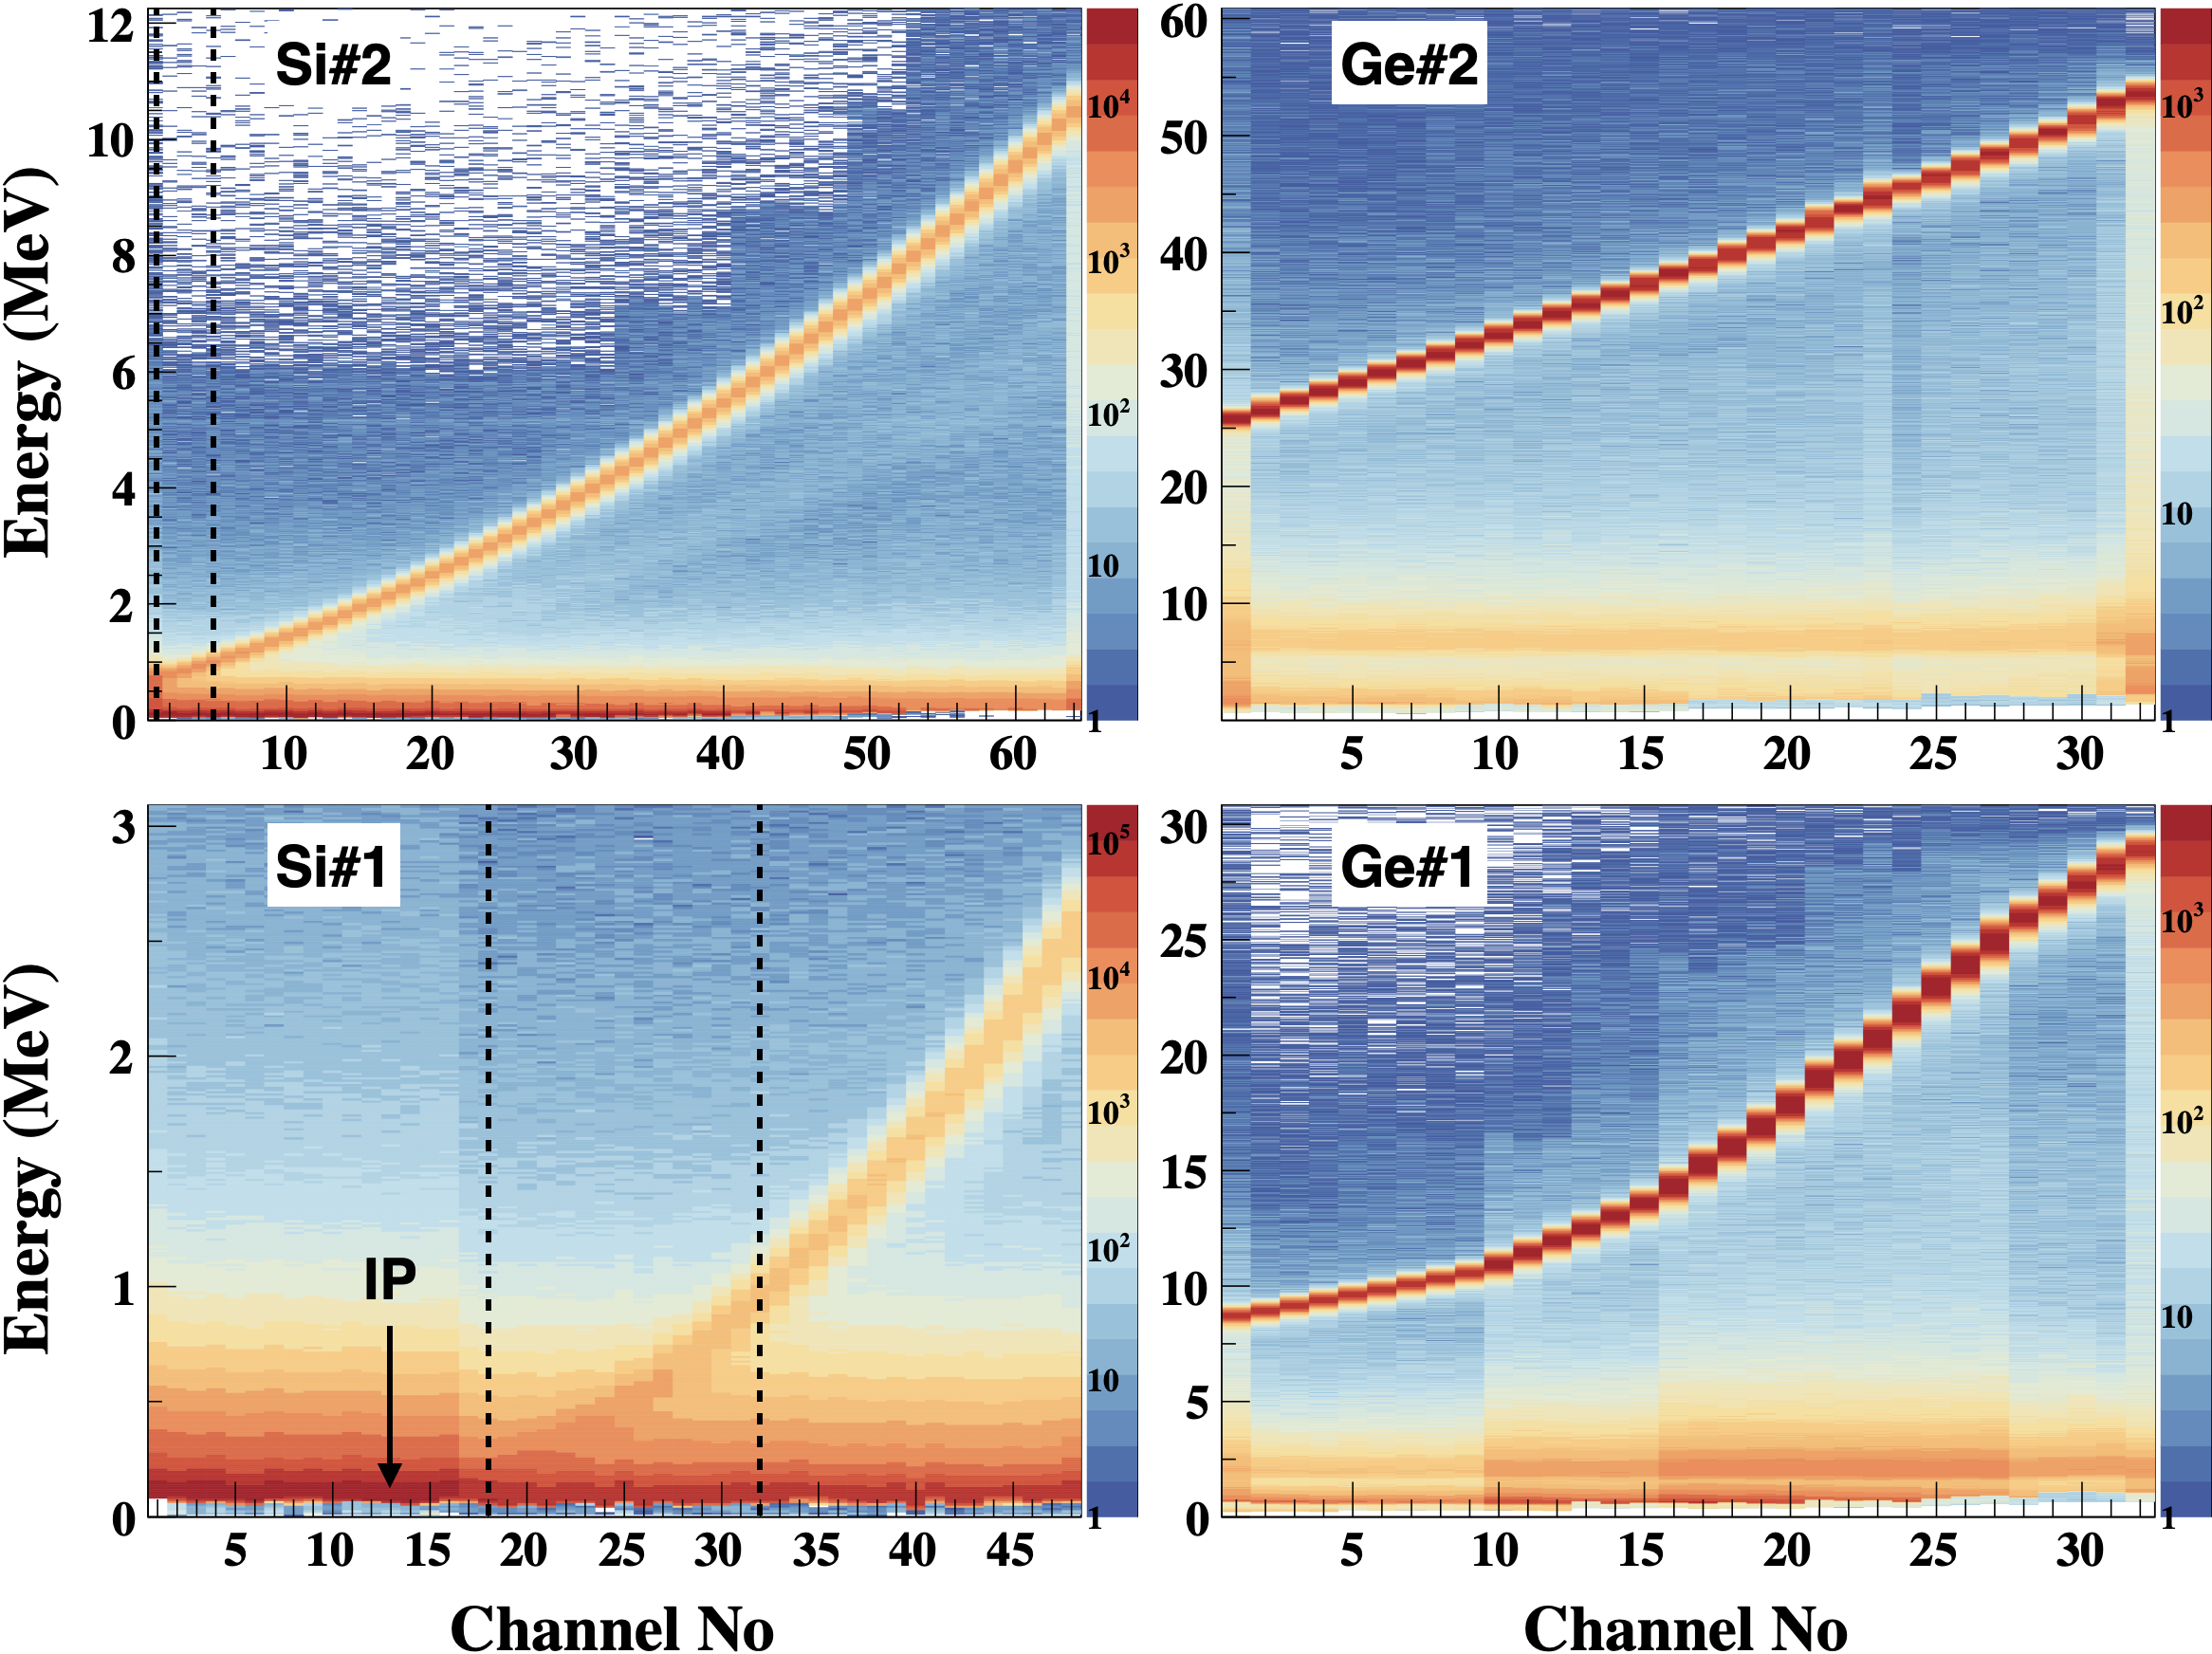
\includegraphics[width=0.48\textwidth]{./energy_vs_strips.png}
  \caption{Energy spectra of all strips of the recoil detector obtained at
    $P_{beam} = 2.2 \si{\momentum}$.}
  \label{fig:energy_vs_strips}
\end{figure}

\par
\medskip

%%%%% Method 1: Combined fit 
For all strips of Ge\#1, Ge\#2 and most strips of Si\#2, a combined fit with
a three-component background model and an elastic peak model is used to extract
the number of elastic events.
The elastic peak is described by the so-called Crystal-Ball function\cite{r1}, which
is composed of a Gaussian core and a power-law tail on each side of the core.
The three components in the background model are: 1) a
fast-decreasing exponential component, which has very high yield at low energy; 2)
a slow-decreasing exponential component, which extends to very high energy; 3) a
minimum-ionizing-particle (MIP) component, which is described by a Landau
distribution.
A typical result using this fit model is shown in Fig. \ref{fig:combined_fit}.
The MIP events are mainly generated by the pions from inelastic interactions,
which have a most probable energy deposit of \SI{0.37}{\MeV} in Si\#1 and Si\#2,
\SI{2.2}{\MeV} in Ge\#1 and \SI{7.0}{\MeV} in Ge\#2.
The accuracy of this method deteriates when the elastic peak is close to the MIP
peak, and both peaks are embeded among the large low-energy background.
In this case, it's hard to estimate the parameters of each component separately
and thus a large error exists in determining the fraction of each background component.
\begin{figure}[!htb]
	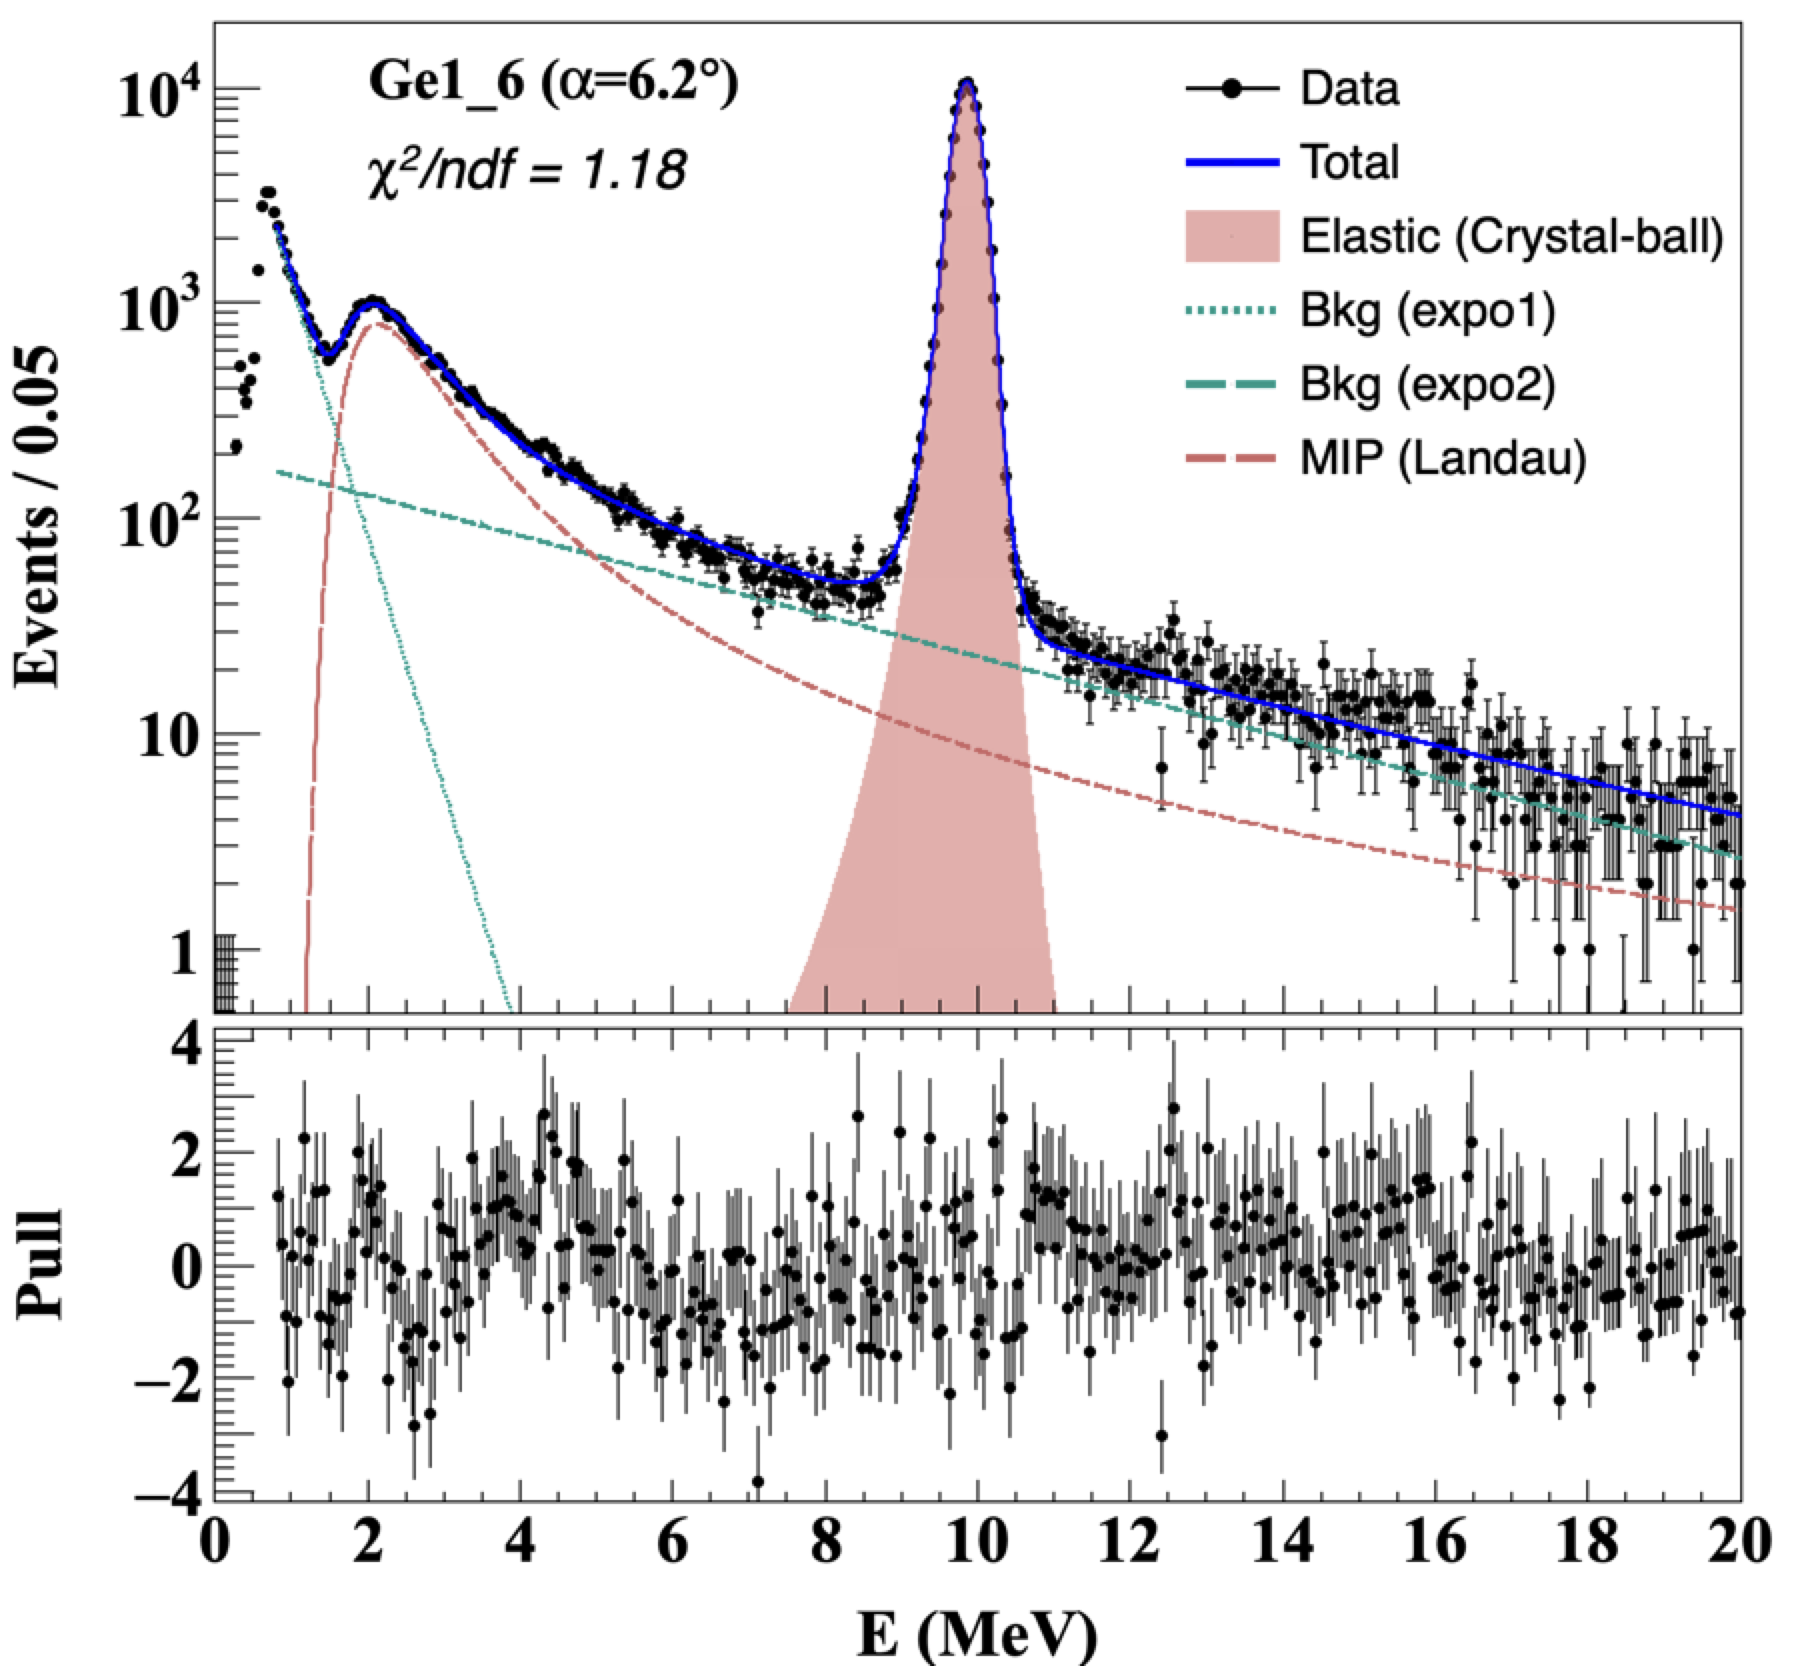
\includegraphics[width=0.45\textwidth]{./combined_fit.png}
  \caption{An example of the combined fit of the total energy spectrum for a strip at large recoil angle.}
  \label{fig:combined_fit}
\end{figure}

% \enlargethispage{-\baselineskip}
\par
\medskip

%%%%% Method 2: TOF-E selection
For recoil strips at small recoil angles ($\alpha$), the low-energy background
can be selectively supressed by using the TOF-E relation of the recoil proton in
coincidence with the forward scattered particle.
The energy spectra from three strips at different recoil angles are shown in
Fig. \ref{fig:coulomb_cb2_fit},  before and after the TOF-E selection.
The remaining background after this selection comes from elastic scattering off the residual gas.
The shape of this background is well described by the Coulomb elastic scattering cross
section, due to the uniform distribution of the residual gas \cite{r2} and the
rapid decrease of the elastic scattering cross section beyond the Coulomb region.
Thus, the extraction of the yield of elastic events from the target body is carried out
using a combined fit of a Coulomb elastic scattering formula and the Crystal-Ball
function.
The results of this fit for the three strips are also shown in Fig. \ref{fig:coulomb_cb2_fit}.
However, this method is constrained by the limited acceptance of the forward detector:
1) below the lower limit, the full target body isn't covered as shown in Fig.
\ref{fig:coulomb_cb2_fit} (a);
2) beyond the upper limit, the full beam profile isn't covered as shown in
Fig. \ref{fig:coulomb_cb2_fit} (c).
Only a few strips on Si\#1 and Si\#2 can use this method to extract all
elastic scattering events from the beam-target interaction, see Fig. \ref{fig:coulomb_cb2_fit} (b).
\begin{figure}[!htb]
	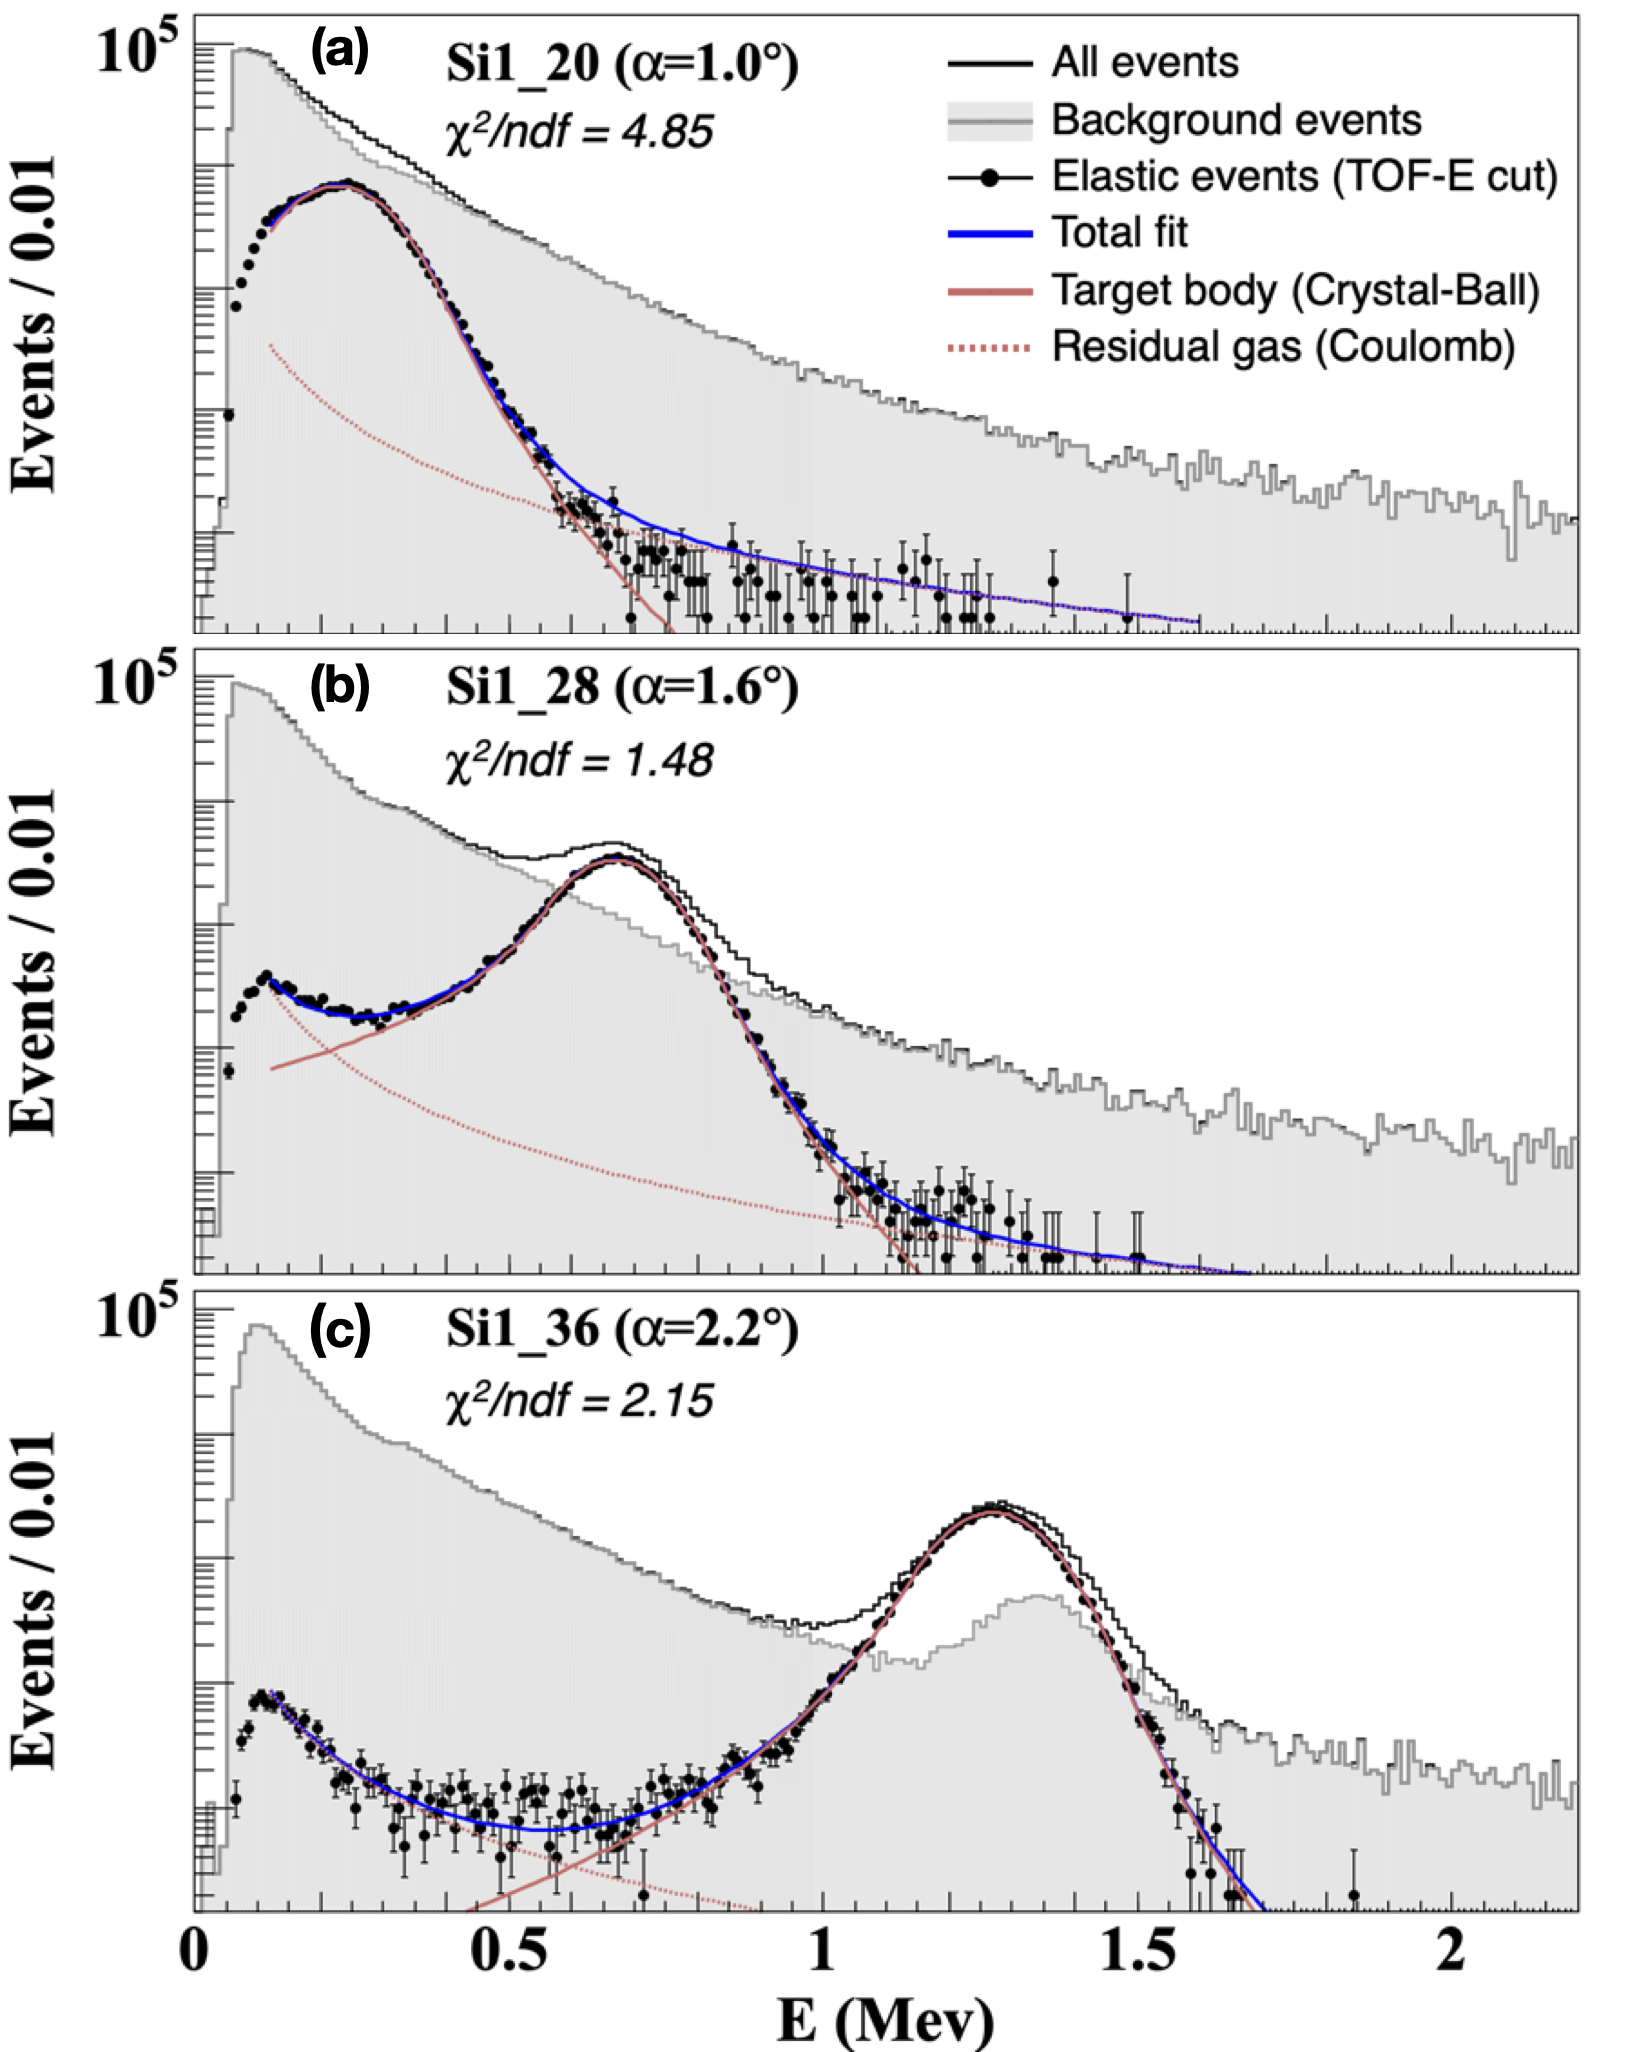
\includegraphics[width=0.45\textwidth]{./coulomb_cb2_fit.png}
  \caption{The energy spectra of TOF-E selected events (black dots) from strips at three
    recoil angles. The black lines are from all events and the grey areas are the
  supressed background events. }
  \label{fig:coulomb_cb2_fit}
\end{figure}

\par
\medskip

%%%%% Method 3: Background substraction
A third method is used to extract the rate of elastic events on those strips of
Si\#1 and Si\#2 that are not fully covered by the forward detector or the
elastic peak is not well separated from the MIP peak or low-energy background.
First, a background model is determined from the strips which are fully covered by the forward detector.
The elastic peak in these strips is already substracted using the second method, thus generating 
pure inelastic background spectra, which are used as the background model
for the other strips in the same sensor.
This background model is combined with the Crystal-Ball function to fit the full
energy spectrum and extract the yield of elastic events.
An example of the fit result for the same channel in Fig. \ref{fig:coulomb_cb2_fit}
(c) is shown in Fig. \ref{fig:bkg_vs_tofe}, in which the fitted background component is substracted. 
\begin{figure}[b!]
  \centering
	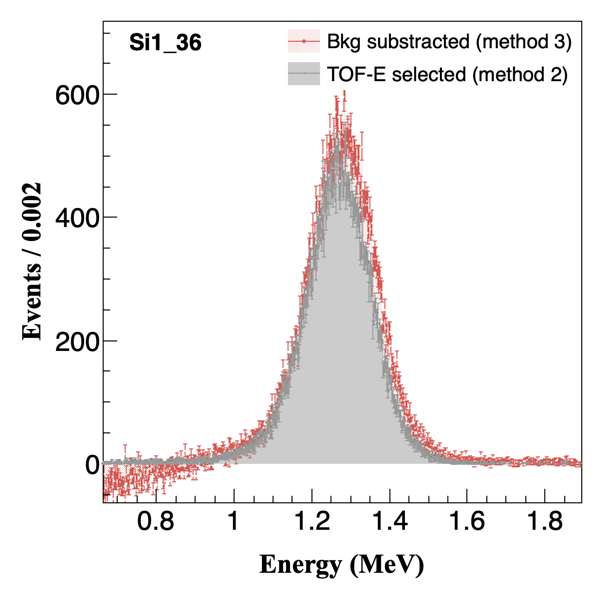
\includegraphics[width=0.4\textwidth]{./bkg_vs_tofe.png}
  \caption{Comparison of the elastic peak extracted using method 3 (red) and
    the TOF-E selected elastic peak using method 2 (grey).}
  \label{fig:bkg_vs_tofe}
\end{figure}
Comparing to the TOF-E selected elastic peak, the full elastic peak can now be extracted.
This method can be applied on all strips on Si1/Si2.
However, the systematic error becomes larger for strips located at very small
recoil angle and far away from the strips, which are used for the extraction of the background model.

\par
\medskip

%%%%% Discussion: Consistency between 3 methods: 3 VS 1, 3 VS 2
The consistency of the different extraction methods is checked by comparing the
ratio of the number of events under the extracted elastic peak of the same recoil strip.
Two groups of strips from Si\#1 and Si\#2 respectively are selected for the
comparison between method 2 and 3, and one group of strips from Si\#2 are selected
for the comparison between method 1 and 3.
The results are summarized in Fig. \ref{fig:extraction_consistence}.
For all studied strips, the relative difference in yield between the methods is
less than \SI{0.6}{\percent}, indicating excellent consistency.
The increasing discrepancy at low and high recoil energies between method 2 and
method 3 on Fig. \ref{fig:extraction_consistence} (a) is due to the limited
acceptance of the forward detector.
The fully-covered strips on Si\#1 and Si\#2 can also be identified based on this comparison.
\begin{figure}[!htb]
	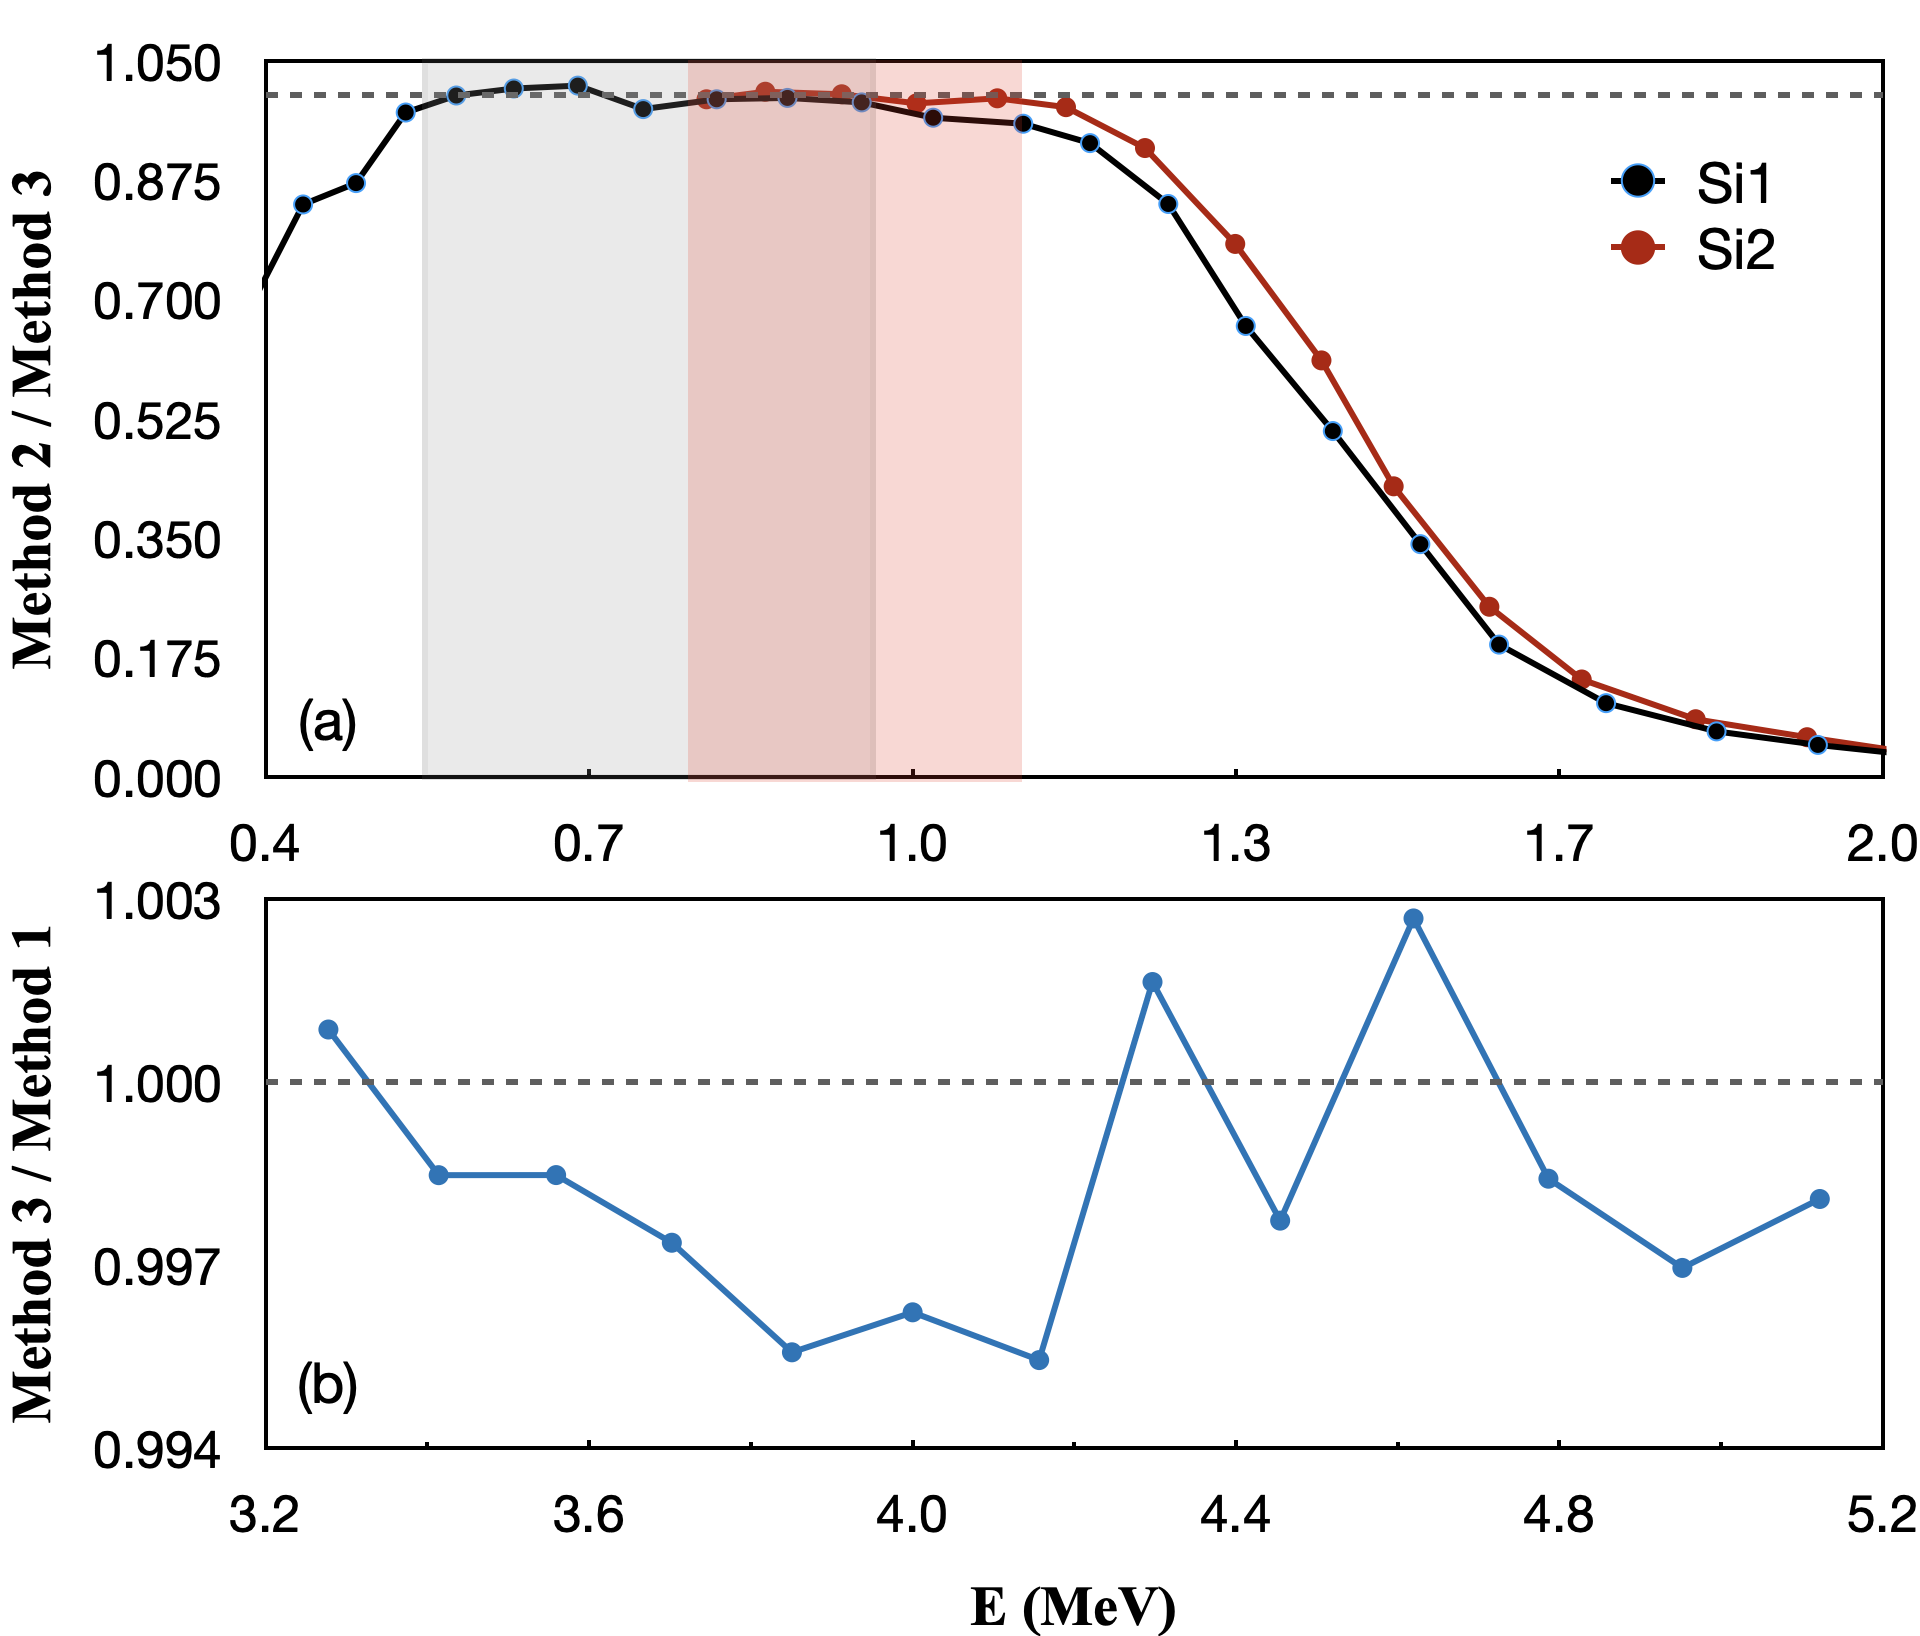
\includegraphics[width=0.5\textwidth]{./comparison_methods.png}
  \caption{Comparison between the different extraction
    methods: a) the ratio of elastic scattering event yield between method 2 and
    method 3, the shaded regions show the fully-covered strips on Si\#1
    (black) and Si\#2 (red), respectively; b) the ratio of the elastic yield for
    method 3 to method 1 in the higher energy reange.}
  \label{fig:extraction_consistence}
\end{figure}

\par
\medskip

%%%%% Conclusion
Three methods of extracting the yield of elastic scattering from the total
energy spectrum are studied and compared.
The Crystal-Ball function is adopted as the reponse function of a single recoil strip to the
elastic scattering events from the target body.
The three methods differ by processing the background components differently.
Although these methods are consistent with each other, it's found that they are best suited for
processing strips located at different recoil angles, to achieve the best accuracy
and smallest error.
No single method is suitable for processing all recoil strips.
The extracted yield of elastic events from these methods can be used as
the essential input data set for the determination of the differential cross-section in the further analysis.

\par
\medskip

%----------------------------------------------------------------
\begin{thebibliography}{99}
\bibitem{r1}
  \href{https://www.slac.stanford.edu/cgi-bin/getdoc/slac-r-255.pdf}{J. E.
    Gaiser, Appendix-F Charmonium Spectroscopy from Radiative Decays of the J/Psi and Psi-Prime, Ph.D. Thesis, SLAC-R-255 (1982).}
\bibitem{r2} Y. Zhou, Determination of the cluster target density profile in KOALA, IKP Annual Report 2021.
\end{thebibliography}
\end{document}

